\documentclass[a4paper,12pt]{article}

\usepackage{amsmath,amssymb,multicol,tikz,enumitem}
\usepackage[margin=2cm]{geometry}
\usetikzlibrary{calc,shapes}

\pagestyle{empty}

\newcommand\N{\mathbf{N}}
\newcommand\Q{\mathbf{Q}}
\newcommand\R{\mathbf{R}}
\newcommand\Z{\mathbf{Z}}

\usepackage{array}
\newcolumntype{P}[1]{>{\centering\arraybackslash}p{#1}}
\newcommand\indd{${}$\hspace{20pt}}

\begin{document}

\begin{center}
\parbox{3.5cm}{\textbf{Data Structures}} \hfill {\bf\Huge Worksheet 6} \hfill \parbox{3.5cm}{\flushright\textbf{BITL2}} \\[5pt]
\rm\small 21 October 2021
\end{center}

\hrule\vspace{2pt}\hrule

\vspace{10pt}
\noindent
Recall that a \textbf{red-black} tree satisfies the following properties:
\begin{itemize}
\item The root and all leaves are black
\item Both children of a red node are black
\item All leaves have the same black depth (black ancestors)
\end{itemize}
\hrule

\begin{enumerate}

\item \textbf{Warm up 1:} Answer the following True / False statements about red-black trees.
\begin{enumerate}
\item A subtree of a red-black tree is itself a red-black tree.
\item The sibling of a leaf is either a leaf or it is red.
\item Every red-black tree is an AVL (height-balanced) tree.
\end{enumerate}

\vfill
\item A \textbf{matching} of a tree is a subset of the edges of a tree so that no two edges share a vertex. A matching is \textbf{perfect} if every vertex of the tree is incident to exactly one edge of the matching.
\begin{enumerate}
\item Does a complete binary tree always have a matching? Which do and which do not?
\item For a binary tree of height $h$, what is the largest number of nodes it can have to have a perfect matching?
\item For an $n$-ary tree of height $h$, what is the largest number of nodes it can have to have a perfect matching?
\end{enumerate}

\vfill
\item Recall the \textbf{insertion} sort, \textbf{selection} sort, \textbf{merge} sort, and \textbf{quick} sort algorithms.
\begin{enumerate}
\item Which of these are in-place algorithms? Deterministic algorithms?
\item If an input list is already sorted, which algorithm will be fastest?
\item How many comparisons do each of insertion and selection sort do in each step, when sorting the list below? A comparison is when two list elements are compared in size.
\[
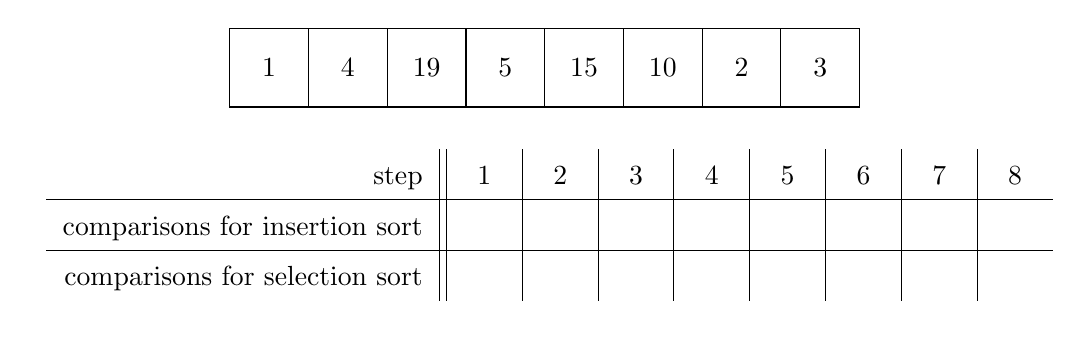
\begin{tikzpicture}
\foreach \x\n in {1/1, 2/4, 3/19, 4/5, 5/15, 6/10, 7/2, 8/3}{
  \node at (\x,0) {\n};
  \path[draw] (\x-.5,-.5) rectangle (\x+.5,.5);
}
\node at (4.5,-2) {
\renewcommand\arraystretch{1.5}
\begin{tabular}{r||c|c|c|c|c|c|c|c}
step & \phantom{a}1\phantom{a} & \phantom{a}2\phantom{a} & \phantom{a}3\phantom{a} & \phantom{a}4\phantom{a} & \phantom{a}5\phantom{a} & \phantom{a}6\phantom{a} & \phantom{a}7\phantom{a} & \phantom{a}8\phantom{a}\\\hline
comparisons for insertion sort & & & & & & & &\\\hline
comparisons for selection sort & & & & & & & &
\end{tabular}};
\end{tikzpicture}
\]
\item Draw all the steps that merge sort would take on this list.
\item For quick sort, which of the values in the list are good pivots? Draw all the steps that quick sort would take on the list, if the pivot is element number $\lfloor\frac{\text{length of list}}{2}\rfloor$.
\end{enumerate}


\end{enumerate}

\end{document}